% !TeX root = ../main.tex
% Add the above to each chapter to make compiling the PDF easier in some editors.

\chapter{Groups}\label{cha:groups}
\section{Groups and Homomorphisms}
\begin{defn}[Semigroup, Monoid, and Group]\leavevmode
\begin{enumerate}[(a),leftmargin=2\parindent]
    \item A set $G$ with a mapping $\cdot$ on $G$ (that is, $\cdot: G \times G \to G$) is named \begin{itemize}
        \item \emph{semigroup}\index{semigroup} if $\forall a, b, c \in G.\ (a \cdot b) \cdot c = a \cdot (b \cdot c)$; \margintag{\emph{associativity}\index{associativity}}
        \item \mbox{\emph{monoid}\index{monoid} if it is a semigroup and $\exists e \in G.\ \forall a \in G.\ e \cdot a = a \cdot e = a$; \margintag{$e$ is called \emph{neutral element}\index{neutral element}}}
        \item \emph{group}\index{group} if it is a monoid and $\forall a \in G.\ \exists a' \in G.\ a \cdot a' = a' \cdot a = e$. \margintag{$a'$ is the \emph{inverse element}\index{inverse element} of $a$}
    \end{itemize}
    
    \item A group $(G,\cdot)$ is named \emph{abelian}\index{abelian group} or \emph{commutative}\index{commutativity} if the group operation $\cdot$ is commutative under elements of $G$, \begin{align}
        \forall a, b \in G.\quad a \cdot b = b \cdot a.
    \end{align}
    
    \begin{marginfigure}
        We denote groups by $(G,\cdot)$. If the group operation $\cdot$ is clear from context, we refer to the group simply as $G$. Subsequently, we also write $a b$ instead of $a \cdot b$.
    \end{marginfigure}
\end{enumerate}
\end{defn}

\begin{rmk}
Let $G$ be a group. Then, \begin{enumerate}[(a),leftmargin=2\parindent]
    \item there is exactly one neutral element $e \in G$ and for every $a \in G$ there is exactly one inverse element $a' \in G$, which we call $\inv{a}$;
    \item the mapping on $G$, which we refer to by $\cdot$, may be resembled by any symbol;
    \item if $G$ is abelian, often \begin{itemize}
        \item $+$ is used instead of $\cdot$,
        \item $0$ is used instead of $e$, and
        \item $-a$ is used instead of $\inv{a}$.
    \end{itemize}
\end{enumerate}
\end{rmk}

\begin{ex}{Semigroups, monoids, and groups}{}
\begin{center}
\setlength\tabcolsep{5pt}
\begin{tabular}{lrrrrr}
\toprule
 & $(\NO,+)$ & $(\NZ,+)$ & $(\Z,+)$ & $(\Z,\cdot)$ & $(\woZ{\Q},\cdot)$ \\
 \midrule
 semigroup & yes & yes & yes & yes & yes \\
 \addlinespace
 monoid & no & yes & yes & yes & yes \\
 \addlinespace
 group & yes & no & yes & no & yes \\
 \bottomrule
\end{tabular}
\end{center}
\end{ex}

\begin{ex}{General linear and special linear group}{}
The \emph{general linear group}\index{general linear group} $\GL{n}{K}$ is the group of invertible\marginfootnote{Recall from linear algebra that a matrix $\mA$ is invertible iff $\determ{\mA} \neq 0$.} ${n \times n}$ linear maps over a field\marginfootnote[1\baselineskip]{A \emph{field}\index{field} is a set of elements with well-defined operations for addition, subtraction, multiplication, and division. We give a formal definition in \cref{defn:field}. Examples of fields are the rational numbers $\Q$, the real numbers $\R$, and the complex numbers $\C$.} $K$, \begin{align}
    \GL{n}{K} \defeq \{\mA \in K^{n \times n} \mid \determ{\mA} \neq 0\}.
\end{align}

The \emph{special linear group}\index{special linear group} $\SL{n}{K}$ is the group of normed linear maps over the field $K$, \begin{align}
    \SL{n}{K} \defeq \{\mA \in K^{n \times n} \mid \determ{\mA} = 1\}.
\end{align}

The group operation of $\GL{n}{K}$ and $\SL{n}{K}$ is matrix multiplication. Their neutral element is the identity matrix $\mI$, and the inverse elements are the matrix inverses $\inv{\mA}$.
\end{ex}

\begin{ex}{Abelian groups}{}
\begin{itemize}
    \item $(\Z,+)$
    \item $(\Q,+)$
    \item $(\R,+)$
    \item $(\woZ{\R},\cdot)$
\end{itemize}
\end{ex}

\begin{ex}{Symmetric group}{}
The \emph{symmetric group}\index{symmetric group} $S_n$ is the group of bijections on the set $[n]$, \begin{align}
    S_n \defeq \{\sigma : [n] \to [n] \mid \text{$\sigma$ is bijective}\},
\end{align} with the function composition ``$\circ$'' as mapping.

Elements of the symmetric group ${\sigma \in S_n}$ are called \emph{permutations}\index{permutation}. The neutral element of the symmetric group is the identity $\id$, which maps each input to itself.

There are multiple ways of representing permutations. Perhaps the most natural representation of ${\sigma \in S_n}$ is a mapping in \emph{two-line notation}\index{two-line notation}, \begin{align}
    \sigma = \begin{pmatrix}
        1 & 2 & \cdots & n \\
        \sigma(1) & \sigma(2) & \cdots & \sigma(n) \\
    \end{pmatrix},
\end{align} or in \emph{one-line notation}\index{one-line notation} by simply omitting the first line, \begin{align}
    \sigma = (\sigma(1)\ \sigma(2)\ \cdots\ \sigma(n)).
\end{align}

An alternative characterization of a permutation is as a product of (disjoint) cycles. A \emph{cycle}\index{cycle} ${\rho \in S_n}$ is a permutation that maps a subset of numbers ${\{i_1, i_2, \dots, i_r\} \subseteq [n]}$ in a cyclic fashion. That is, \begin{align}
    \rho(i_1) = i_2,\quad \rho(i_2) = i_3,\quad \cdots\quad \rho(i_{r-1}) = i_r,\quad \rho(i_r) = i_1,
\end{align} leaving all other ${j \in [n]}$ fixed. We denote such a cycle by \begin{align}
    \rho = (i_1\ i_2\ \cdots\ i_r).
\end{align} A cycle of length $r$, is also called \emph{$r$-cycle}. 2-cycles are called \emph{transpositions}\index{transposition}.

Every permutation ${\sigma \in S_n}$ can be written as a ``product'' (i.e., composition), \begin{align}
    \sigma = \rho_1 \cdots \rho_s,
\end{align} where $\rho_i$ are cycles with pairwise disjunct elements. This is also known as the \emph{cycle notation}\index{cycle notation} of $\sigma$. Note that the ordering of $\rho_1, \dots \rho_s$ does not matter, as their elements are disjoint.

The cycle lengths $r_1, \dots, r_s$ (in descending order) of $\rho_1, \dots, \rho_s$ are the \emph{cycle type}\index{cycle type} of $\sigma$.

\begin{rmk}
The symmetric group is not abelian.
\end{rmk}\vspace{-20pt}\begin{proof}
We have $(1\ 2)(2\ 3) = (2\ 3\ 1)$ and $(2\ 3)(1\ 2) = (1\ 3\ 2)$.
\end{proof}
\end{ex}

\begin{lem}[Notation and Rules]
Let $(G,\cdot)$ be a group. \begin{enumerate}[(a),leftmargin=2\parindent]
    \item For $a \in G, n \in \NZ$, we write \begin{itemize}
        \item $a^n \defeq \underbrace{a \cdot a \cdots a}_{\text{$n$ many}}$,
        \item $a^0 \defeq e$, and
        \item $a^{-n} \defeq \underbrace{\inv{a} \cdot \inv{a} \cdots \inv{a}}_{\text{$n$ many}}$.
    \end{itemize}
    
    \item $\forall a, b \in G.\ \forall m, n \in \Z.$ \begin{enumerate}[(i)]
        \item $\inv{(\inv{a})} = a$
        \item $a^m \cdot a^n = a^{m+n}$, $(a^m)^n = a^{m \cdot n}$
        \item $\inv{(a \cdot b)} = \inv{b} \cdot \inv{a}$
    \end{enumerate}
\end{enumerate}
\end{lem}
\begin{proof}[Proof of (b)(iii)] $(a \cdot b) \cdot \inv{b} \cdot \inv{a} = a \cdot \underbrace{(b \cdot \inv{b})}_{=e} \cdot \inv{a} = a \cdot \inv{a} = e$.
\end{proof}

\begin{defn}[Subgroup]
A subset $U \subseteq G$ is called a \emph{subgroup}\index{subgroup} of a group $G$ (denoted $U \leq G$) if $U$ itself is a group with mapping $\cdot$. That is, $U$ is a subgroup iff \begin{enumerate}[(a),leftmargin=2\parindent]
    \item $e \in U$; \margintag{$U$ contains the neutral element}
    \item $\forall a, b \in U.\quad a \cdot b \in U$; and \margintag{the mapping $\cdot$ is closed wrt. $U$}
    \item $\forall a \in U.\quad \inv{a} \in U.$ \margintag{the mapping $\inv{(\dots)}$ is closed wrt. $U$}
\end{enumerate} Associativity follows from $G$ being a group.
\end{defn}

\begin{ex}{Subgroups}{}
\begin{itemize}
    \item $\{e\}, G \leq G$ (\emph{trivial subgroups}\index{trivial subgroups})
    \item $\SL{n}{K} \leq \GL{n}{K}$
    \item Let $2\Z \defeq \{2m \mid m \in \Z\}$, then $(2\Z,+) \leq (\Z,+)$
\end{itemize}
\end{ex}

\begin{rmk}\label{rmk:cap_subgroup}
If $\{U_i\}_{i \in I}$ are subgroups of $G$, then $\bigcap_{i \in I} U_i \leq G$.
\end{rmk}

\begin{defn}[Generated Subgroup]
For any $M \subseteq G$, \begin{align}
    \gen{M} \defeq \bigcap_{\substack{U \leq G \\ M \subseteq U}} U \leq G, \margintag{by \cref{rmk:cap_subgroup}}
\end{align} is the \emph{subgroup generated by $M$}\index{generated subgroup}. In particular, $\gen{M}$ is the ``smallest'' subgroup that includes $M$.
\end{defn}

\begin{lem}
For $M \neq \emptyset$, we have \begin{align}
    \gen{M} = \{a_1 \cdot a_2 \cdots a_n \mid n \in \N, \text{$a_i \in M$ or $\inv{a_i} \in M$}\}.
\end{align}
\end{lem} \begin{proof}[Proof (sketch)]\leavevmode
Let $N \defeq \{a_1 \cdot a_2 \cdots a_n \mid n \in \N, \text{$a_i \in M$ or $\inv{a_i} \in M$}\}$.
\begin{enumerate}[(i),leftmargin=2\parindent]
    \item \underline{$\gen{M} \subseteq N$}: $N \leq G$ and $M \subseteq N \implies \gen{M} \subseteq N$ \margintag{using that $\gen{M}$ is the smallest subgroup including $M$}
    \item \underline{$N \subseteq \gen{M}$}: if $U \leq G$ with $M \subseteq U$, then $U$ includes all of these products $\implies N \subseteq U \implies N \subseteq \gen{M}$ \qedhere
\end{enumerate}
\end{proof}

\begin{ex}{Generated subgroup}{}
$S_3 = \{\id, \underbrace{(1\ 2)}_{\tau_1}, \underbrace{(1\ 3)}_{\tau_2}, \underbrace{(2\ 3)}_{\tau_3}, \underbrace{(1\ 2\ 3)}_{\sigma_1}, \underbrace{(1\ 3\ 2)}_{\sigma_2}\} = \gen{\{\underbrace{(1\ 2)}_{\tau_1}, \underbrace{(1\ 2\ 3)}_{\sigma_1}\}}$.
\end{ex}

\begin{defn}[Cyclic Group]
A group $G$ is \emph{cyclic}\index{cyclic group} if $\exists a \in G$ with \begin{align}
    G = \gen{a} \defeq \gen{\{a\}} = \{a^m \mid m \in \Z\}.
\end{align} Such an $a \in G$, is called a \emph{generator}\index{generator} of $G$.
\end{defn}

\begin{ex}{Cyclic groups}{}
\begin{itemize}
    \item $\gen{i} = \{i^m \mid m \in \Z\}$ is a cyclic subgroup of $(\woZ{\C},\cdot)$, \begin{align*}
        \gen{i} &= \{\dots, \underbrace{i^{-2}}_{=-1}, \underbrace{i^{-1}}_{=-i}, 1, i, \underbrace{i^2}_{=-1}, \underbrace{i^3}_{=-i}, \underbrace{i^4}_{=1}, \underbrace{i^5}_{=i}, \dots\} \\
                &= \{1, i, -1, -i\}.
    \end{align*}
    \item $(\Z,+) = \gen{1} = \{\dots, -2, -1, 0, 1, 2, \dots\}$ is cyclic
\end{itemize}
\end{ex}

\begin{marginfigure}
    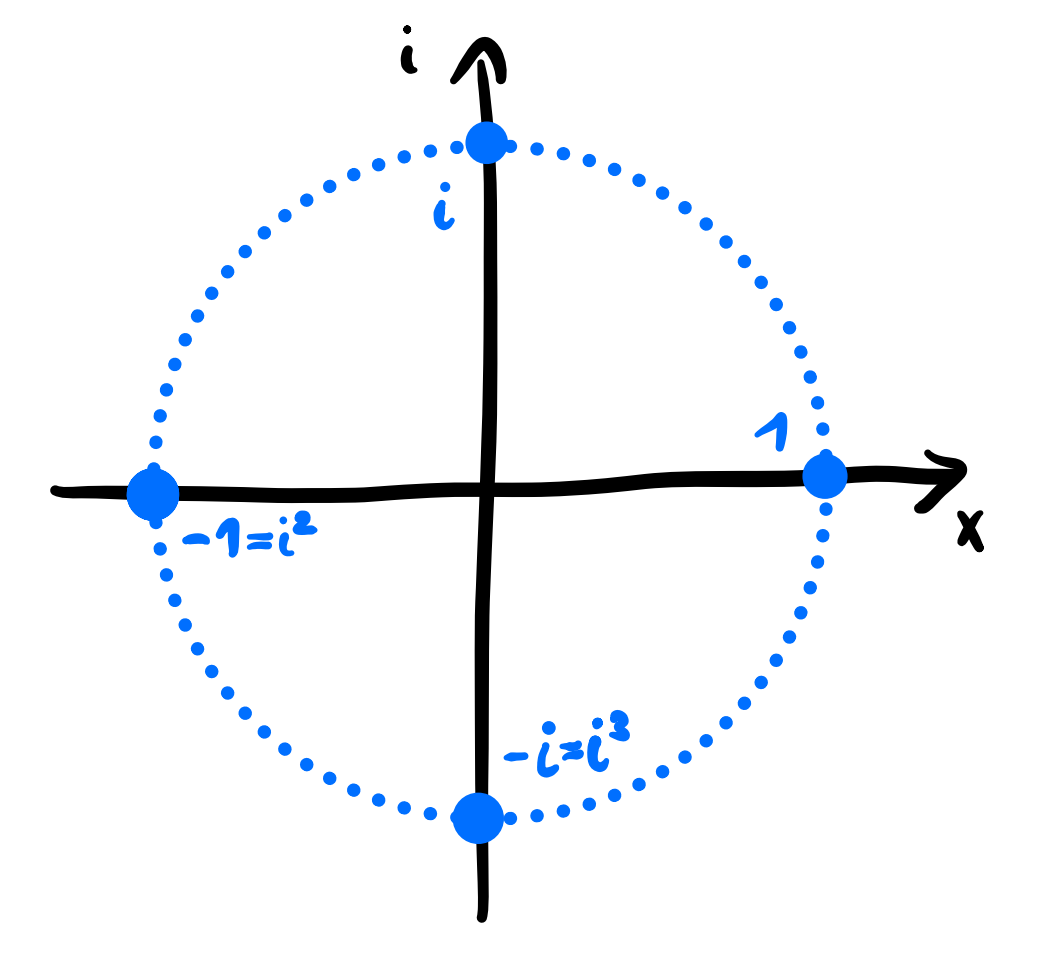
\includegraphics[width=\textwidth]{c_cyclic_subgroup.png}
    \caption{An illustration of the cyclic subgroup $\gen{i}$ in the complex plane.}
\end{marginfigure}

\begin{defn}[Order]

\end{defn}

\section{Normal Subgroups and Quotient Groups}
\section{Homomorphism and Isomorphism Theorems}
\section{Group Actions}
\section{Sylow Theorems}
\section{Direct products and Abelian Groups}
\section{Solvable Groups}
